% ============================================================
%  TERM PROJECT – PROPOSAL
%  Databases · THGA Bochum
%  VPN Access Manager
% ============================================================
\documentclass[11pt,a4paper]{article}

\usepackage{thga-db}
\usepackage{caption}

\renewcommand{\thgaKurs}{Databases}
\renewcommand{\thgaDatum}{Summer Term 2026}
\newcommand{\authorName}{Rayen Ben Haj Rhouma}
\newcommand{\projectTitle}{VPN Access Manager}

\begin{document}
\thispagestyle{empty}
\thgaTitel{Term Project – Proposal}{\projectTitle}

\begin{infobox}
\textbf{Author:} \authorName \\
\textbf{Module:} Introduction to Database Management Systems · THGA Bochum \\
\textbf{Submitted to:} Stephan Bökelmann · \href{mailto:sboekelmann@ep1.rub.de}{sboekelmann@ep1.rub.de} \\
\textbf{Planned effort:} approximately 40 hours over no more than two months
\end{infobox}

% ============================================================
\section{Application domain and motivation}
% ============================================================

Companies that let employees work remotely run one or more VPN gateways so that
staff can reach internal systems over an encrypted tunnel. The IT team needs to
know who is connected right now, to which gateway, from which client IP, and how
much traffic each session used. This matters for capacity planning (a gateway
has a limited number of concurrent slots) and for basic auditing (which user
connected when). Doing this by hand or in a spreadsheet is unreliable: a
spreadsheet cannot guarantee that a user or gateway actually exists, cannot stop
the same session being closed twice, and cannot answer ``how many users are
active on each gateway'' without manual counting.

The proposed application is a small \emph{VPN Access Manager}. It replaces the
spreadsheet with a relational database, a REST API, and a desktop frontend. It
manages \textbf{departments}, \textbf{VPN users}, \textbf{gateways}, and the
\textbf{connection sessions} that link a user to a gateway. Each session records
its status, the client IP, the connect and disconnect times, and the number of
bytes transferred.

\textbf{Usage scenario 1.} An administrator opens the frontend and starts a new
session for a user on the Frankfurt gateway. The system refuses the connection
if that gateway has already reached its maximum number of concurrent sessions.

\textbf{Usage scenario 2.} A capacity manager wants an overview. The main screen
lists every gateway with its region, the number of currently active sessions,
and its maximum, so that gateways close to their limit can be seen at a glance.

% ============================================================
\section{Data model -- ER sketch}
% ============================================================

\begin{figure}[ht]
  \centering
  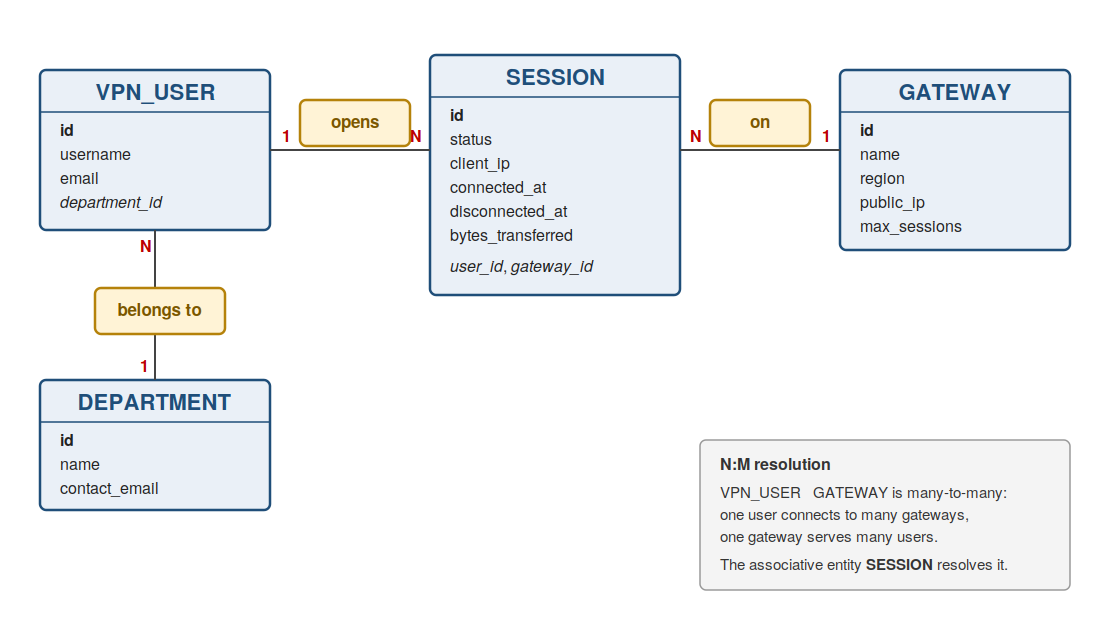
\includegraphics[width=0.95\linewidth]{er-sketch.png}
  \caption{ER model of the VPN Access Manager: entity types, key attributes,
  foreign keys, relationships and cardinalities. The N:M relationship between
  \texttt{vpn\_user} and \texttt{gateway} is resolved by the associative entity
  \texttt{session}.}
  \label{fig:er}
\end{figure}

Figure~\ref{fig:er} shows four entity types. A \texttt{department} groups
employees. A \texttt{vpn\_user} is a person allowed to use the VPN and belongs
to one department. A \texttt{gateway} is a VPN server in a given region with a
maximum number of concurrent sessions. A \texttt{session} is one connection of a
user to a gateway and stores the connection-specific data.

A department \emph{has} many users (1:N) and a user \emph{opens} many sessions
(1:N). The central relationship is between \texttt{vpn\_user} and
\texttt{gateway}: one user can connect to many gateways over time, and one
gateway serves many users, so \texttt{vpn\_user} and \texttt{gateway} form an
\textbf{N:M} relationship. The associative entity \texttt{session} resolves this
N:M relationship into two 1:N relationships and holds the data specific to a
single connection (status, client IP, times, bytes).

% ============================================================
\section{From model to schema}
% ============================================================

The relational schema is derived directly from the ER diagram. Primary keys are
underlined and foreign keys are written in italics.

\begin{itemize}
  \item \texttt{department}(\underline{id}, name, contact\_email)
  \item \texttt{vpn\_user}(\underline{id}, username, email, \emph{department\_id})
  \item \texttt{gateway}(\underline{id}, name, region, public\_ip, max\_sessions)
  \item \texttt{session}(\underline{id}, status, client\_ip, connected\_at,
        disconnected\_at, bytes\_transferred, \emph{user\_id}, \emph{gateway\_id})
\end{itemize}

The database uses the following integrity constraints:

\begin{itemize}[topsep=2pt]
  \item \texttt{vpn\_user.username} and \texttt{gateway.name} are unique.
  \item \texttt{status} is restricted to \texttt{active} or \texttt{closed} by a
        CHECK constraint.
  \item \texttt{disconnected\_at} must be NULL while the session is
        \texttt{active} and must not be earlier than \texttt{connected\_at}.
  \item \texttt{user\_id} and \texttt{gateway\_id} are foreign keys with
        referential integrity.
  \item A gateway must not hold more \texttt{active} sessions than its
        \texttt{max\_sessions} (enforced by the API before insert).
\end{itemize}

\textbf{Normalisation.} The schema is in third normal form (3NF). Each table
describes one subject, every non-key attribute depends only on its table's
primary key, and no non-key attribute depends transitively on another.
Department data is stored once in \texttt{department} and referenced through
\texttt{department\_id}; gateway data is stored once in \texttt{gateway} and
referenced through \texttt{gateway\_id}; \texttt{session} stores only the data
specific to a single connection.

% ============================================================
\section{API design}
% ============================================================

The REST API is implemented with FastAPI. Read operations require no API key.
Write operations require a valid \texttt{X-API-Key} header. Request bodies are
validated with Pydantic models, and SQL queries use parameters rather than
string concatenation.

\renewcommand{\arraystretch}{1.2}
\begin{tabularx}{\linewidth}{@{}p{2cm}p{4.6cm}X@{}}
\toprule
\textbf{Method} & \textbf{Path} & \textbf{Purpose} \\
\midrule
\texttt{GET}  & \texttt{/gateways}               & List gateways with region and a count of active sessions (JOIN + aggregation) \\
\texttt{GET}  & \texttt{/sessions}               & List sessions with user, department, gateway, status, times (multiple JOINs); optional filters \\
\texttt{GET}  & \texttt{/sessions/\{id\}}        & Return the full details of one session \\
\texttt{POST} & \texttt{/sessions}               & Open a session after validating FKs and the gateway capacity limit (X-API-Key) \\
\texttt{POST} & \texttt{/sessions/\{id\}/close}  & Set an active session to \texttt{closed} and record the disconnect time (X-API-Key) \\
\bottomrule
\end{tabularx}

For example, \texttt{GET /sessions?status=active\&gateway=gw-eu-1} returns only
the active sessions on one gateway. The endpoint \texttt{GET /gateways} joins
\texttt{gateway} and \texttt{session}, filters for active sessions, and groups
by gateway to compute the number of active sessions per gateway.

% ============================================================
\section{Frontend prototype (hand sketches)}
% ============================================================

The frontend is a Python/tkinter desktop application. It talks only to the REST
API and never connects to PostgreSQL directly. At startup a connection dialog
asks for the API URL and the \texttt{X-API-Key}; the key is kept in memory for
the session and never written to disk. The main window offers a gateway
overview plus access to the session list, the open-session form, and the close
action.

\begin{figure}[ht]
\centering
\begin{minipage}[t]{0.47\linewidth}\centering
  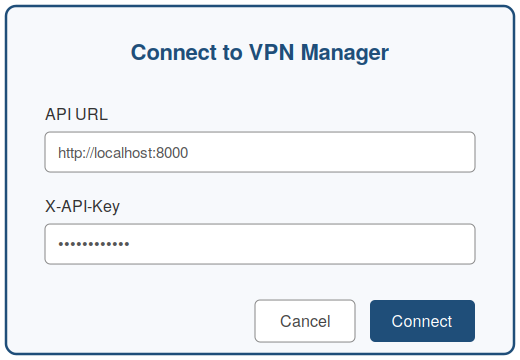
\includegraphics[width=\linewidth]{fe-connect.png}
  \captionof{figure}{Startup connection dialog: API URL + X-API-Key.}
  \label{fig:fe-connect}
\end{minipage}\hfill
\begin{minipage}[t]{0.47\linewidth}\centering
  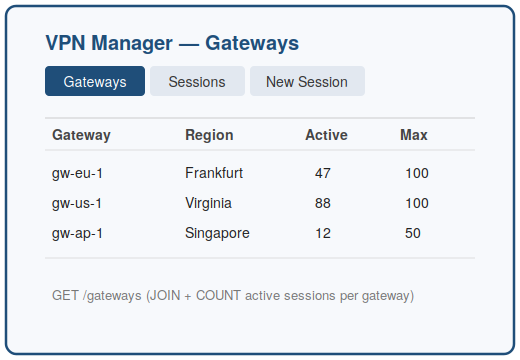
\includegraphics[width=\linewidth]{fe-main.png}
  \captionof{figure}{Main screen: gateway overview, calls \texttt{GET /gateways}.}
  \label{fig:fe-main}
\end{minipage}

\vspace{1em}

\begin{minipage}[t]{0.47\linewidth}\centering
  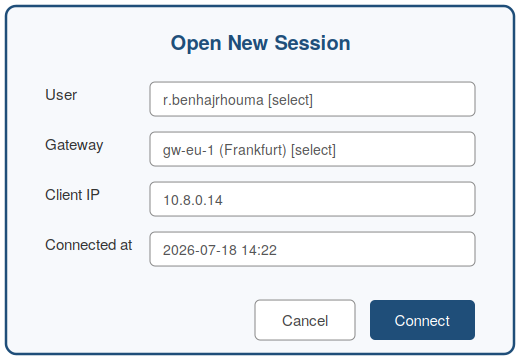
\includegraphics[width=\linewidth]{fe-detail.png}
  \captionof{figure}{Open-session form: calls \texttt{POST /sessions}.}
  \label{fig:fe-detail}
\end{minipage}\hfill
\begin{minipage}[t]{0.47\linewidth}\centering
  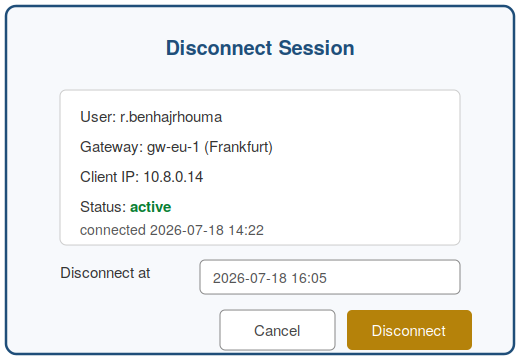
\includegraphics[width=\linewidth]{fe-second.png}
  \captionof{figure}{Disconnect confirmation: calls \texttt{POST /sessions/\{id\}/close}.}
  \label{fig:fe-second}
\end{minipage}
\end{figure}

Figures~\ref{fig:fe-connect}--\ref{fig:fe-second} show the four screens of the
prototype. Figure~\ref{fig:fe-connect} shows the connection dialog that collects
the API URL and \texttt{X-API-Key} at startup; Figure~\ref{fig:fe-main} shows
the gateway overview populated by \texttt{GET /gateways}; Figure~\ref{fig:fe-detail}
shows the form that opens a new session via \texttt{POST /sessions}; and
Figure~\ref{fig:fe-second} shows the confirmation step that closes a session via
\texttt{POST /sessions/\{id\}/close}.

% ============================================================
\section{Operation with Docker Compose}
% ============================================================

The backend consists of two containers orchestrated with Docker Compose. The
\texttt{postgres} service creates the schema and seed data from an
\texttt{init.sql} script on first start. The \texttt{api} service is built from
the \texttt{api/} directory, waits for a healthy database via a health check,
and exposes FastAPI on port 8000.

Database credentials and the API key are read from a \texttt{.env} file that is
excluded from Git; a committed \texttt{.env.example} documents the required
variables with placeholder values. Deployment on the lecture server is:
(1)~copy \texttt{.env.example} to \texttt{.env} and set secure values;
(2)~run \texttt{docker compose up -d -\/-build};
(3)~verify with \texttt{docker compose ps} and the API health endpoint;
(4)~install the frontend with \texttt{sudo dpkg -i vpn-manager\_0.1.0\_amd64.deb};
(5)~launch \texttt{vpn-manager} and enter the API URL and key. The frontend is
bundled with PyInstaller and packaged as a \texttt{.deb} with fpm.

% ============================================================
\section{Scope, milestones and risks}
% ============================================================

\textbf{Scope.} The minimum viable product contains four tables, five REST
endpoints, one tkinter desktop application with four screens, Docker Compose
deployment, automated tests, documentation, and a short demonstration video.
Real VPN authentication, live traffic capture, per-user roles, and historical
reporting dashboards are explicitly outside the scope.

\textbf{Milestones and schedule.}

\renewcommand{\arraystretch}{1.2}
\begin{tabularx}{\linewidth}{@{}p{1.4cm}Xp{1.8cm}@{}}
\toprule
\textbf{Week} & \textbf{Milestone} & \textbf{Est. hours} \\
\midrule
1     & Final ER model, SQL schema, constraints, seed data, local Docker Compose setup & 8 \\
2--3  & FastAPI models and all endpoints, X-API-Key guard, JOIN and aggregation queries & 12 \\
4--5  & tkinter frontend, API integration, validation, Debian packaging & 12 \\
6     & Automated tests, deployment verification, documentation, video & 8 \\
\bottomrule
\end{tabularx}

\textbf{Risks and mitigation.}
\begin{itemize}[topsep=2pt]
  \item \textbf{Capacity-rule risk:} the ``do not exceed \texttt{max\_sessions}''
        check is the one non-trivial business rule; it is implemented in the API
        before insert and covered by a dedicated unit test early.
  \item \textbf{Packaging risk:} PyInstaller/fpm may miss dependencies;
        packaging is tested in a clean Debian environment, not left to the end.
  \item \textbf{Deployment risk:} the API may start before PostgreSQL is ready;
        Docker health checks and service dependencies handle this.
\end{itemize}

% ============================================================
\section{Acceptance criteria and testing}
% ============================================================

\textbf{Acceptance criteria.}
\begin{itemize}[topsep=2pt]
  \item The database starts from a clean Docker volume and creates all tables,
        constraints, and seed records without manual SQL.
  \item Opening a session for a non-existent user or gateway is rejected with a
        documented 4xx response.
  \item Opening a session on a gateway that is already at \texttt{max\_sessions}
        is rejected.
  \item \texttt{GET /gateways} returns the correct active-session count for
        every gateway, including gateways with zero active sessions (JOIN +
        aggregation).
  \item \texttt{GET /sessions} correctly applies the \texttt{status} and
        \texttt{gateway} filters.
  \item Write endpoints return HTTP 401 when the API key is missing or invalid.
  \item Closing a session sets it to \texttt{closed} and records the disconnect
        time, and a second close attempt does not change it again.
\end{itemize}

\textbf{Test plan.}
\begin{itemize}[topsep=2pt]
  \item \textbf{Database:} verify PK/FK/UNIQUE/CHECK constraints and the
        time-ordering rule against a disposable test database.
  \item \textbf{API:} use \texttt{pytest} and FastAPI's \texttt{TestClient}
        for happy paths and error cases on all five endpoints.
  \item \textbf{Business rule:} a test that fills a gateway to its
        \texttt{max\_sessions} and asserts that one more open request returns a
        4xx --- this covers the capacity-rule risk named above.
\end{itemize}

\vspace{1em}
\begin{infobox}
\textbf{Effort budget:} the whole term project (system, documentation and video)
is designed to fit into roughly \textbf{40\,h of work} over at most
\textbf{2 months}.
\end{infobox}

\end{document}
